\documentclass{article}

\usepackage[dvips]{graphicx}
\usepackage[dvips]{color}

\pagestyle{plain}
\textwidth 17.2cm
\textheight 26cm
\oddsidemargin -0.9cm
\topmargin -1.8cm
\begin{document}
\centerline{\Large{\bf Proposed Autoguider Integration Changes}}
\vspace*{0.2cm}
\centerline{\Large History}
\begin{center}
\begin{tabular}{|l|l|l|p{20em}|}
\hline
{\bf Version} & {\bf Author} & {\bf Date} & {\bf Notes} \\
\hline
0.1 & I.A. Steele & 11/01/07  & First draft \\
\hline
0.2 & R.J. Smith & 25/01/07 & Typos\\
\hline
0.3 & S.N. Fraser & 26/01/07 & Generally updated and more typos.\\
\hline
0.4 & C.J.Mottram & 02/04/07 & More typos, first go at TOCA implementation.\\
\hline
\end{tabular}
\end{center}
\newpage
\tableofcontents
\listoffigures
\listoftables

\section{Introduction}

A meeting was held between IAS, CJM, RJS and SNF on 10th Jan 2006
to discuss proposed autoguider integration changes.  This
document records the output of that meeting.

There are currently several systems that issue
commands to/from the autoguider with different
associated logic.
 
This is confusing from an operations point of view, and causes
problems such as the need to re-acquire the guide
star after each MULTRUN (e.g. when a filter change
occurs).

\section{Current Configurations}

\subsection{SCA}

An {\rm Observation} can be set in the OSS to three different
autoguider modes:

\begin{itemize}
\item OFF
\item MAYBE
\item ALWAYS
\end{itemize}

Autoguide ON is always issued by the Instrument at the
start of a MULTRUN.

The RCS configures the ISS whether or not to forward autoguider control requests. 
If acquisition fails for an ALWAYS observation, 
the observation fails and a veto is sent back to the OSS to disable this group for a period 
(the autoguider may be working later) and a {\em different} {\rm Observation}
is picked from the OSS. For a MAYBE observation the exposure is re-attempted with 
autoguider control forwarding disabled.

Autoguide OFF is always issued by the Instrument at the
end of the MULTRUN, this is always forwarded.

\subsection{BGCA}

A config file may be set to indicate whether or not
to use the autoguider, and the RCS configures the ISS
whether or not to pass on the commands from the instrument.

\subsection{PCA}

There is currently no method of controlling this
via the PCA. 

\subsection{TOCA}

The AUTOGUIDER is controlled by explicit TOCA
commands, (AUTO ON and AUTO OFF) that are passed on by the RCS.

\subsection{Manual Observing}

On entry to ENGINEERING state (i.e. manual observing) forwarding of
Autoguider commands is disabled, these must be then issued via the TCS.

\section{Proposed New Configuration}

The instruments no longer issue AUTOGUIDER ON 
or OFF commands.

All autoguider commands are issued from the ISS.
This allows a single method of using the 
autoguider for all modes. 

The RCS or the Manual Observer has two commands
it can send to the ISS:

\begin{itemize}
\item START\_AUTOGUIDING
\item STOP\_AUTOGUIDING
\end{itemize}

When the ISS receives the START\_AUTOGUIDING command,
it will attempt to start guiding.  The ISS will
return GUIDING once it starts guiding or
FAILED if it can't guide for some reason (the
autoguider is broken, it can't find a guide star
etc.)  

During guiding the ISS may need to turn the autoguider on or
off as necessary (e.g. if it receives an OFFSET (from an instrument)) 
if we are not implementing them with a working TWEAK command).  
When this happens it should send an INTERRUPTED notification back to the
RCS/Manual Observer.  Once guiding resumes it should
send back a RESUMED notification.  If it fails to resume (timeout?)
it should send back a FAILED notification.  FAILED can also be
sent back at any time during guiding if a problem occurs.
 
From the point of view of the current JMS protocol the RCS (or GUI) issuing the
START\_AUTOGUIDING command would expect a DONE message to confirm that autoguiding has started
or a FAILED message to indicate failure to acquire, the additional INTERRUPTED and RESUMED
messages would arrive after this - which is not permitted by the protocol, I would therefore
expect to implement an asynchronous callback from the ISS to the RCS/GUI - for information only
as the RCS has nothing to do in this instance anyway though a manual user might be interested
to know that the ISS has stopped and restarted autoguiding. In the case of a FAIL during autoguiding,
i.e. after successful acquire this would also have to go via asynchronous callback and in this case the
RCS would want to know.


For each Agent then we have:

\subsection{SCA}

Assuming autoguider is required for an {\rm Observation} the RCS will need to issue the START\_AUTOGUIDING at start of the {\rm Observation}.  If the {\rm Group} contains multiple targets the RCS will need to issue the appropriate START\_AUTOGUIDING and STOP\_AUTOGUIDING associated with slews, rotator changes and mosaic offsets.  
Where observations are consecutive of the same target (without rotator or mosaic offsets), the autoguider should not stop and start in between.  Behaviour for MAYBE as before in terms of the reaction to FAILED. Fig.~\ref{fig:case1} shows a typical use scenario with the SupIRCam making dither offsets while guiding on 2 consecutive targets.

\subsection{BGCA}

Set by a config file (per target?  per observation? or just
overall?). per target seems most logical e.g. sequence like:-

\begin{itemize}
\item Slew onto target 1 and set rotator.
\item START\_AUTOGUIDING to ISS.
\item Config R
\item Expose
\item Config G
\item Expose
\item Config B
\item Expose
\item STOP\_AUTOGUIDING to ISS
\item Track axes off or stop them.
\item Slew onto target 2 and set rotator.
\item START\_AUTOGUIDING to ISS.
\item etc, etc
\end{itemize}


\subsection{PCA}

A new parameter to the CCDFIXED command will be needed
to indicate if the autoguider is to be used definitely/maybe/not.
The PCA should only take notice of it if the PCA is
requesting a SLEW (identified by a negative exposure time)
so that if the autoguider is requested as part of a slew,
it is left running without re-acquisitions through
different colour images.

e.g. CCDFIXED target ra dec ... [MAND\_AUTO $|$ NO\_AUTO $|$ OPT\_AUTO ] 

Note that the autoguider will be left guiding after all images are taken in the same way
that the axes are left tracking - as there is no way to inform the PCA that another set
of observations will not be taking place. 

\subsection{TOCA}

The TOCA commands {\bf AUTO ON} and {\bf AUTO OFF} will now send
{\bf START\_AUTOGUIDING} and {\bf STOP\_AUTOGUIDING} commands to the ISS.
On receipt of an {\bf OFFSET} TOCA command the ISS will automatically {\bf Ag\_off} and 
{\bf Ag\_on} around the Offby as the SCA mode does. 
The TOCA client agent is responsible for issuing {\bf AUTO OFF} before any {\bf SLEW} TOCA command.

The TOCA agent will register a callback for INTERRUPTED/RESUMED/FAILED messages from the ISS. This will
update some internal status query-able by the {\bf STATUS} command. Therefore, a TOCA client agent can monitor
whether autoguiding has failed during an {\bf EXPOSE} command, or in the simplest non multi-threaded case test
the status at the end of the {\bf EXPOSE} to see whether autoguiding failed during that exposure.

\subsection{Manual Observing}

A button on the RCSGui to issue START\_AUTOGUIDING
and STOP\_AUTOGUIDING is required.  If START\_AUTOGUIDING
is used, this allows an \emph{integrated} approach to the
use of the autoguider with instruments.  If not,
then the observer can control the autoguider with the
TCS. 

\newpage

   \begin{figure}[h]
   \begin{center}
   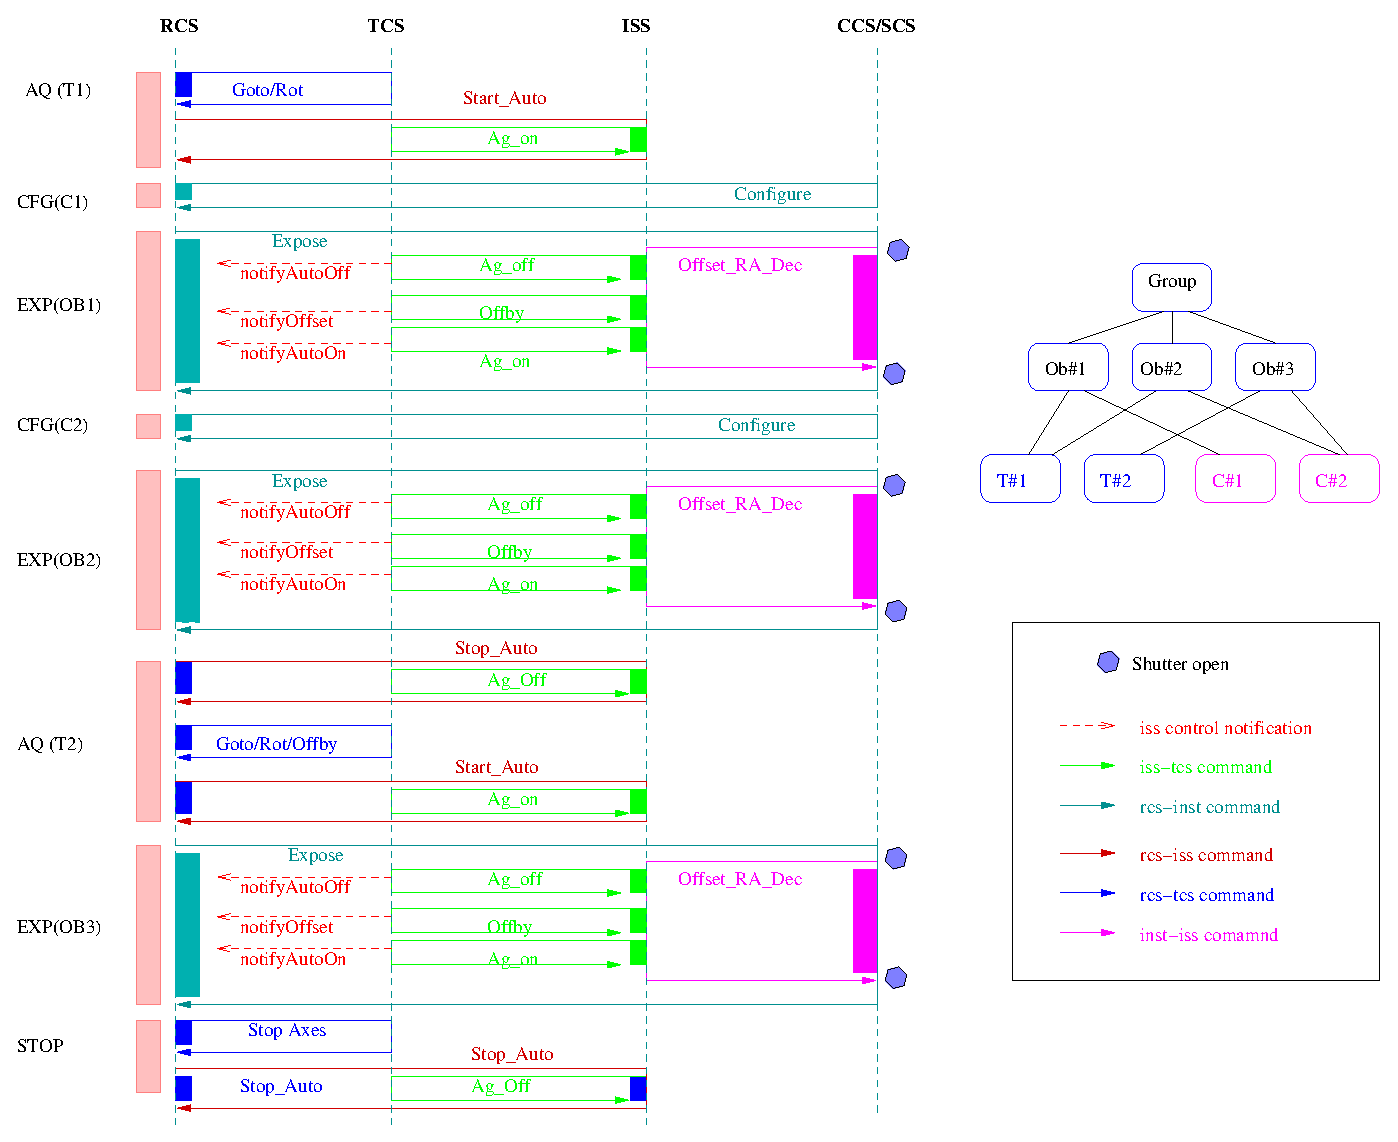
\includegraphics[height=10cm]{iss_ag_case1.eps}
   \end{center}
   \label{fig:case1} 
   \caption[SupIRCam Use case.] 
   {An example of using the autoguider with SupIRCam applied offsets.}
   \end{figure} 


\end{document}



















